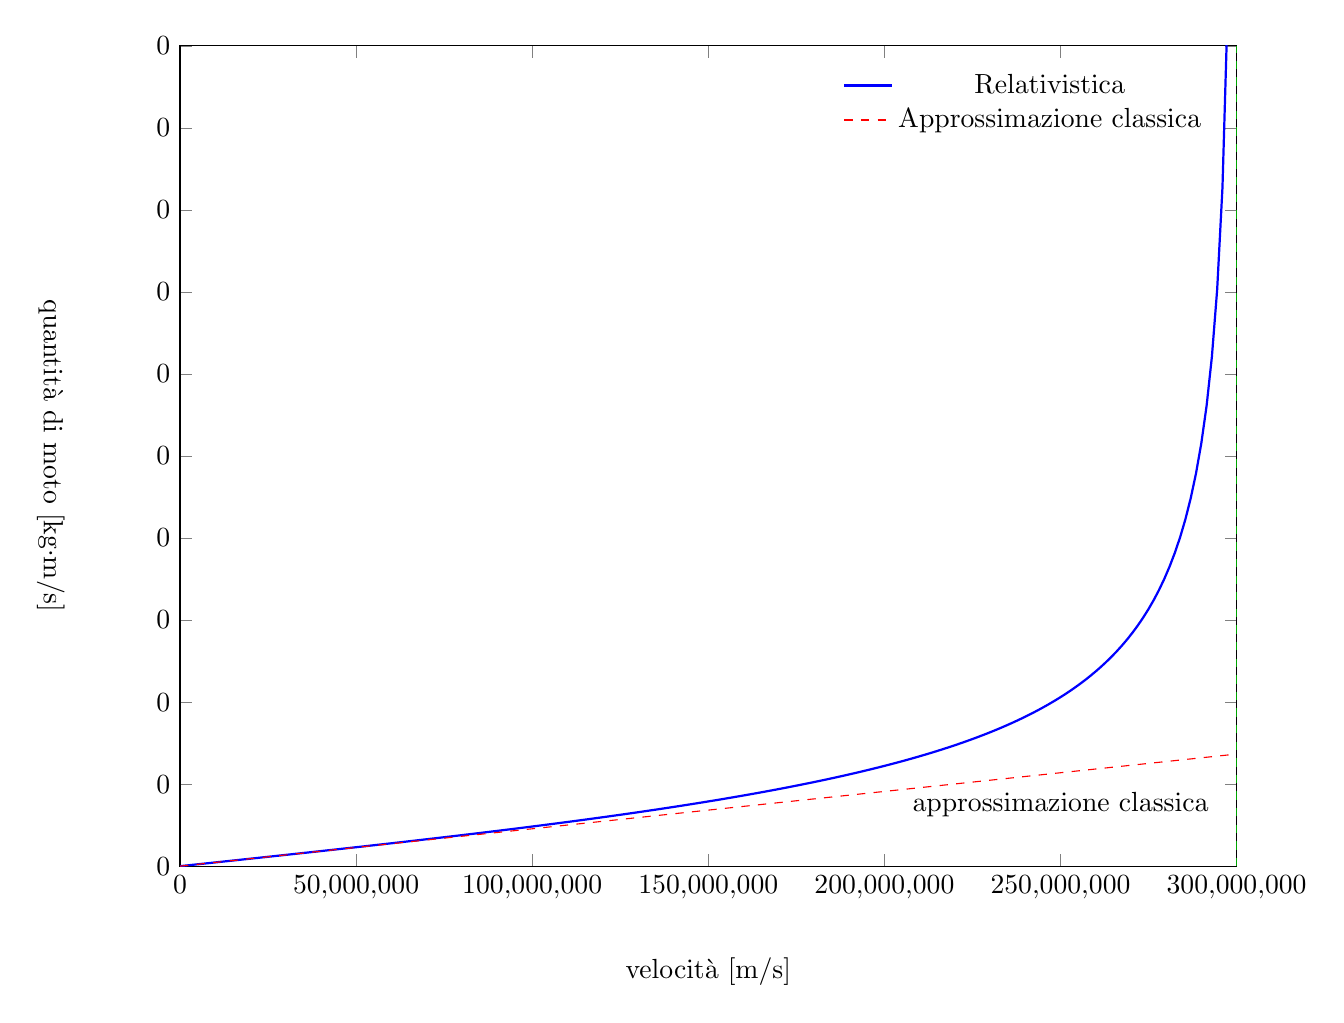
\begin{tikzpicture}
\begin{axis}[
    width=15cm,
    height=12cm,
    xlabel={velocità [m/s]},
    ylabel={quantità di moto [kg$\cdot$m/s]},
    xmin=0, xmax=3e8,
    ymin=0, ymax=2e-21,
    xtick={0,0.5e8,1e8,1.5e8,2e8,2.5e8,3e8},
    xticklabel style={/pgf/number format/fixed},
    yticklabel style={/pgf/number format/fixed},
    scaled y ticks=false,
    scaled x ticks=false,
    y label style={at={(axis description cs:-0.1,.5)},rotate=180},
    x label style={at={(axis description cs:0.5,-0.1)}},
    legend style={draw=none},
]

% Parametri
\def\m{9.11e-31} % massa elettrone
\def\c{3e8}      % velocità della luce

% Curva relativistica
\addplot[blue, thick, domain=0:2.99e8, samples=200] 
    {(\m*x)/sqrt(1-(x/\c)^2)};
\addlegendentry{Relativistica}

% Curva classica
\addplot[red, dashed, domain=0:3e8, samples=100] 
    {\m*x};
\addlegendentry{Approssimazione classica}

% Linea verticale c
\addplot[green, dashed] coordinates {(3e8,0) (3e8,2e-21)};

% Etichetta
\node at (axis cs:2.5e8,1.5e-22) {approssimazione classica};

\end{axis}
\end{tikzpicture}
